\section{Zielsetzung}
In den beiden folgenden Experimenten soll die Ablenkung von Elektronen im elektrischen und magnetischen Feld untersucht werden. Außerdem soll die Stärke des Erdmagnetfeldes bestimmt werden.

\section{Theoretische Grundlage}
\label{sec:Theorie}
\subsection{Aufbau der Kathodenstrahlröhre}
Die beiden Versuche werden in einem Hochvakuum durchgeführt, da die Elektronen sonst mit den Luftmolekülen wechselwirken würden. Dazu wird die Kathodenstrahlröhre (Braunsche Röhre) verwendet. Diese besteht aus drei Hauptkomponenten: der Elektronenkanone, einem Ablenksystem und einem Nachweissystem.\\
\textbf{Die Elektronenkanone:} \\
Die Elektronenkanone erzeugt freie Elektronen durch Glühemission und beschleunigt diese. Da zu wird ein Kathode indirekt beheizt. Diese wird von dem Wehnelt-Zylinder umgeben welcher die Intensität des Elektronenstrahls steuert. Die Elektronen werden durch die nachfolgenden Elektroden beschleunigt. Danach werden die beschleunigten Elektronen Fokussiert. \\
\textbf{Das Ablenksystem:} \\
Das Ablenksystem besteht aus zwei, zueinander parrallelen Kondensatorplatten, welche ein annähernd homogenes elektrisches Feld erzeugen in dem die Elektronen Abgelenkt werden. Sollen die Elektronen in eine weitere Richtung abgelenkt werden wird ein weiteres Plattenpaar um 90 Grad versetzt eingebaut. \\
\textbf{Das Nachweissystem:} \\
Das Nachweissystem visualisiert den auftrefenden Elektronenstrahl.\\
In der nachfolgenden Abbildung wird der Sachverhalt verdeutlicht.

\begin{figure}[H]
	\centering
	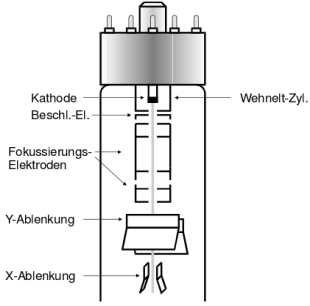
\includegraphics[height=6.5cm]{picture/Kathodenstrahlroehre.PNG}
	\caption{Schematischer Aufbau einer Kathodenstrahlröhre. \cite[2]{V501}}
	\label{fig:Kathode}
\end{figure}

\subsection{Ablenkung von Elektronen im E-Feld}
Zwischen dem Wehnelt-Zylinder und den Beschleunigerelektroden liegt eine hohe Spannung $U_\text{B}$ an, sodass die Elektronen beschleunigt werden. Aus der Energieerhaltung folgt:
\begin{equation}
	\frac{m_0 v^2}{2} = e_0 U_\text{B}
\end{equation}
mit der Elementarladung $e_0$, der Elektronenmasse $m_0$ und der Geschwindigkeit $v$. \\
Durch das ändern der Kondensatorspannung wird die Ablenkung des Elektronenstrahls vergößert oder verkleinert. Diese Ablenkung hängt von der Feldstärke $E$ und der Elektronengeschwindigkeit $v$ ab. Außerdem wird angenommen, dass der Plattenabstand $d$ viel kleiner als die Plattenlänge $p$ ist, somit gilt:
\begin{align*}
	E = \frac{U_\text{d}}{d}
\end{align*}
wobei $U_\text{d}$ der Ablenkspannung entspricht. \\
Unter Betrachtung der Geschwindigkeitskomponenten, dem Winkel $\theta$ der Richtungsänderung und der Abbildung \eqref{fig:AblenkungE} ergibt sich für die Verschiebung $D$:
\begin{equation}
	D = L\theta = \frac{p L U_\text{d}}{2 d U_\text{B}} \propto U_\text{d}
\end{equation}
Mit dem Abstand $L$ zwischen Kondensator und Nachweissystem. \\

\begin{figure}[H]
	\centering
	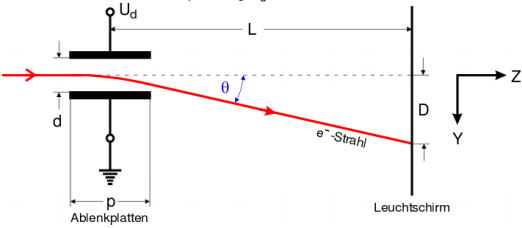
\includegraphics[height=6.5cm]{picture/AblenkungEFeld}
	\caption{Die Ablenkung eines Elektronenstrahls im E-Feld. \cite[3]{V501}}
	\label{fig:AblenkungE}
\end{figure}

Um möglichst genaue Messergebnisse erzielen zu können müssen daher $L$ und $p$ möglichst groß und $U_\text{B}$ möglichst klein gewählt werden. Allerdings können an einer solchen Röhre nur Wechselspannungen mit kleiner Frequenz untersucht werden. Um Wechselspannungenn mit hoher Frequenz zu untersuchen muss eine Kathodenstrahlröhre mit kleinem $p$ und großem $U_\text{B}$ gewählt werden.








\subsection{Fehlerrechnung}
